\chapter{EGGbot}
\section{inspiration}
Three inspirations for this project
·      Eggbot - \url{http://www.instructables.com/id/Plastic-Egg-Bot/}
 
·  	Femi Owolade supported by Nic Hughes ran a session at Mozilla Festival 2016 using the Crumble’s to make a wheeled robot.
 
·  	The junkbot project \url{https://junkbots.blogspot.co.uk/}

\section{Kit}
\begin{itemize}
    \item Kinder Egg (without the Chocolate and toy)
    \item Crumble Controller available at \url{https://redfernelectronics.co.uk/shop/}
    \item 4x Crocodile clips and leads
    \item Battery pack and 3xAA batteris
    \item Vibrating motor or small DC motor with a weight added to the axel
    \item Tape (lots of)
    \item Pens
    \item Paper
    \item Scissors
    \item Glue and Gluegun (optional)
\end{itemize}
\section{Stage1: Fix the vibrating motor into the Egg.}

Put the vibrating motor into the Egg with the motor electrical connections sticking out the bottom larger half of the egg. Make sure the unbalanced load is free to move – this is bit that causes the vibrations needed to move the egg. The motor can be held in place by sticky-tack or strong tape, or glue (when using glue this is done under adult supervision only)

\begin{figure}
    \centering
    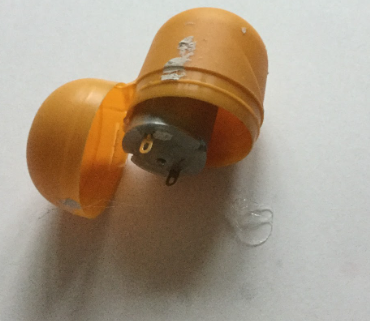
\includegraphics[width=10cm]{chapters/ChapterP1/figures/eggbot_stage1.png}
    \caption{Eggbot drawing stage 1}
    \label{fig:Egggbotdrawing1}
\end{figure}

\section{Stage 2: Sticking the pens on}

This is the trickiest bit. The easiest way to do is cut a strip of tape. Place two pens onto the tape ensuring the pens are the same length from the tape to the nib and the distance between the pens on the tape are far enough apart to place the egg between them.

\begin{figure}
    \centering
    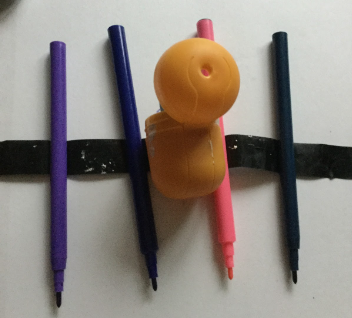
\includegraphics[width=10cm]{chapters/ChapterP1/figures/eggbot_stage2.png}
    \caption{Eggbot drawing stage2}
    \label{fig:Egggbotdrawing2}
\end{figure}

If you are using three pens, the third pen should be placed so that all three form a triangle with equal sides, that means the egg can stand-up on a piece of paper on the pen nibs, without anything supporting it.
 
If you are using four pens, the other two pens should be placed so that all four form a square with equal sides, that means the egg can stand-up on a piece of paper on the pen nibs, without anything supporting it.

\section{Stage 3: Add the battery pack and go.}

Using two wires connecting the battery, to the motors. Remove the nibs and set the bot off. It is hopefully vibrating and shaking and scribbling lines on the paper.

\begin{figure}
    \centering
    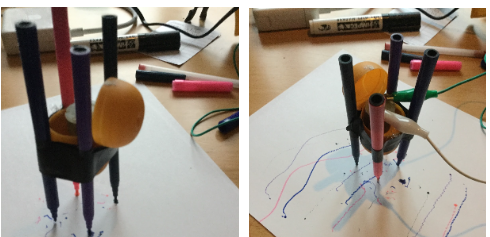
\includegraphics[width=10cm]{chapters/ChapterP1/figures/eggbot_stage3.png}
    \caption{Eggbot drawing stage3}
    \label{fig:Egggbotdrawing3}
\end{figure}


To see one in action go to: 
\url{https://www.youtube.com/watch?v=NRlntdmdQRo}

\section{Stage 3: Add Control (sort of) Crumble}

Disconnect the battery connection (the connections on the motor can stay as they are). Connect the USB cable to the Crumble. To the right of the USB connect there are two connections marked + and -. Connect a Red wire to the + connection and the other end to the red wire of the battery pack. Connect a black wire to the – connection and the other end to the black wire of the battery pack.

\begin{figure}
    \centering
    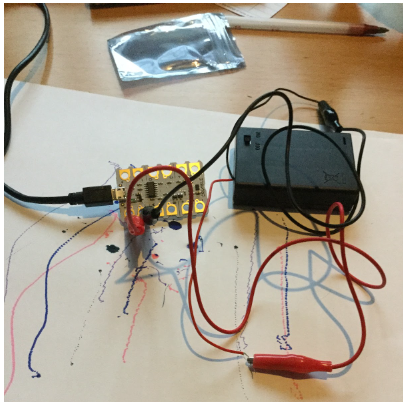
\includegraphics[width=10cm]{chapters/ChapterP1/figures/eggbot_stage4.png}
    \caption{Eggbot drawing with crumble}
    \label{fig:EgggbotdrawingCrumble}
\end{figure}

On the Crumble, on the right-side there are two motor connections connect the Motor to these connections. Don’t worry about which of the motors wires is need you swap them around later.

\begin{figure}
    \centering
    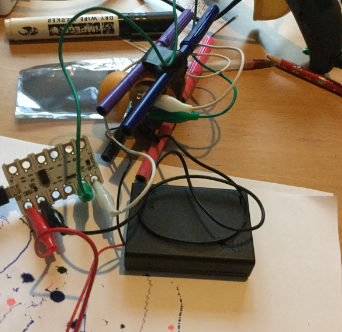
\includegraphics[width=10cm]{chapters/ChapterP1/figures/eggbot_stage5.png}
    \caption{Eggbot and crumble}
    \label{fig:EgggbotdrawingCrumble2}
\end{figure}

\section{Stage 4: ALet's start programming it}

The software can be found at \url{https://redfernelectronics.co.uk/crumble-software/} it includes how to set it up on your own machine.
 
Start the Crumble software. Drag from the left the Program start, motor, and wait blocks. Now join the up start block at the top and the motor block next and the wait block last.


\begin{figure}
    \centering
    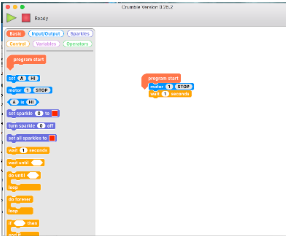
\includegraphics[width=10cm]{chapters/ChapterP1/figures/eggbot_stage6.png}
    \caption{Eggbot and crumble code}
    \label{fig:EgggbotdrawingCrumble3}
\end{figure}

Your code should look like this.

\begin{figure}
    \centering
    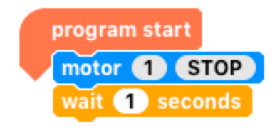
\includegraphics[width=10cm]{chapters/ChapterP1/figures/eggbot_stage7.png}
    \caption{Eggbot and crumble code initial}
    \label{fig:EgggbotdrawingCrumble4}
\end{figure}

Click on the stop within the motor block. It should change to forward. Now you are ready to make it move. Press the green arrow and with the battery pack on, it should (hopefully) keep moving.

\begin{figure}
    \centering
    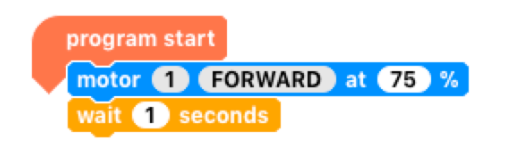
\includegraphics[width=10cm]{chapters/ChapterP1/figures/eggbot_stage8.png}
    \caption{Eggbot and crumble - start}
    \label{fig:EgggbotdrawingCrumble5}
\end{figure}

If you put a second motor block after the wait block with the stop in the block. It such then stop after 1 second of moving.

\section{Stage 5: Making it do more}
.
-   	Drag a do-until block in (found in the control menu).
-   	Go to variable menu and add a new variable, I have used t, select the block marked let=, and drag a t into the blank space.
-   	Drag an increase block onto the screen and drag a t into the blank space.


\begin{figure}
    \centering
    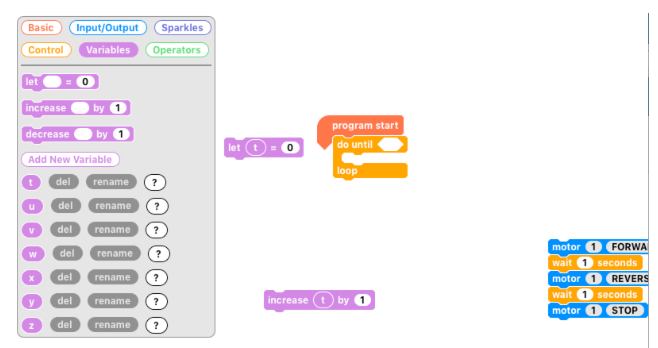
\includegraphics[width=10cm]{chapters/ChapterP1/figures/eggbot_stage9.png}
    \caption{Eggbot and crumble - Lets do a little more}
    \label{fig:EgggbotdrawingCrumbleMore1}
\end{figure}

Go to the operator menu and drag onto the screen an = block, go back to variables menu and drag a t into the first space on the = block and click on the second space on the block and type in 5.

\begin{figure}
    \centering
    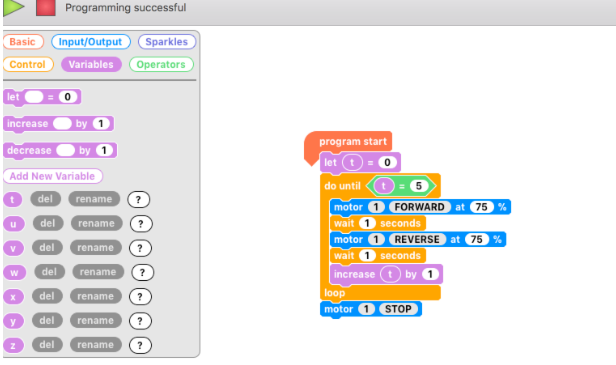
\includegraphics[width=10cm]{chapters/ChapterP1/figures/eggbot_stage10.png}
    \caption{Eggbot and crumble - Lets take it a  little further}
    \label{fig:EgggbotdrawingCrumbleMore2}
\end{figure}

Now for the challenge put all these together to copy what is shown below. Now, put the egg-bot on the paper, with the pen lids off, press the green triangle and the motors should be spun in different directions.
 
This is a junkbot so it may just cause the bot to move a slightly different directions but hopefully it should just draw some squiggly lines.